现在,你坐在哨兵的脑袋里面,你的目标是悄悄摸到敌方基地后面偷家。
但是没认真看规则的你忘记了地图长什么样,你打开手机,发现好心的wzx部长已经帮你存了一份\textbf{标准赛场地图[1]}。
于是你打开\textbf{缺德地图[2]},把赛场地图传上去。你又打开手机GPS,把自己的\textbf{定位[3]}也告诉缺德地图,
最后,你输入目的地,缺德地图就帮你规划好了一条用时最少的路。
于是你就跟着这条路径走,同时你并没有关掉GPS,这样才知道自己有没有走错。
在路上,你在\textbf{视野[4]}里看到了许多其他机器人,你以你秋名山车神的\textbf{车技[5]},在他们之间穿梭,避开了所有车。
突然!What can I say, man!无人机坠机坠在了你前进的道路上。
你对车身大小了如指掌。只看一眼,你计算出哨兵过不去,路被堵了。
鉴于无人机死状惨烈,这无人机短时间是飞不起来,你走不了这条路了。
不过还好,每隔一段时间,缺德地图会再算一次路径,你可能会听到“正在为您重新规划路径”,他帮你找到了另一条路。
虽然“缺德地图持续为您服务”,但是有时候你可能会开到一些“信号不好”,无法获取缺德地图服务的地方。
此时,你要能够在不依靠缺德地图的情况下\textbf{自己找到[6]}信号比较好能重新连接上缺德地图服务的地方。
最终你成功到达了目的地。

\begin{figure}[H]
    \centering
    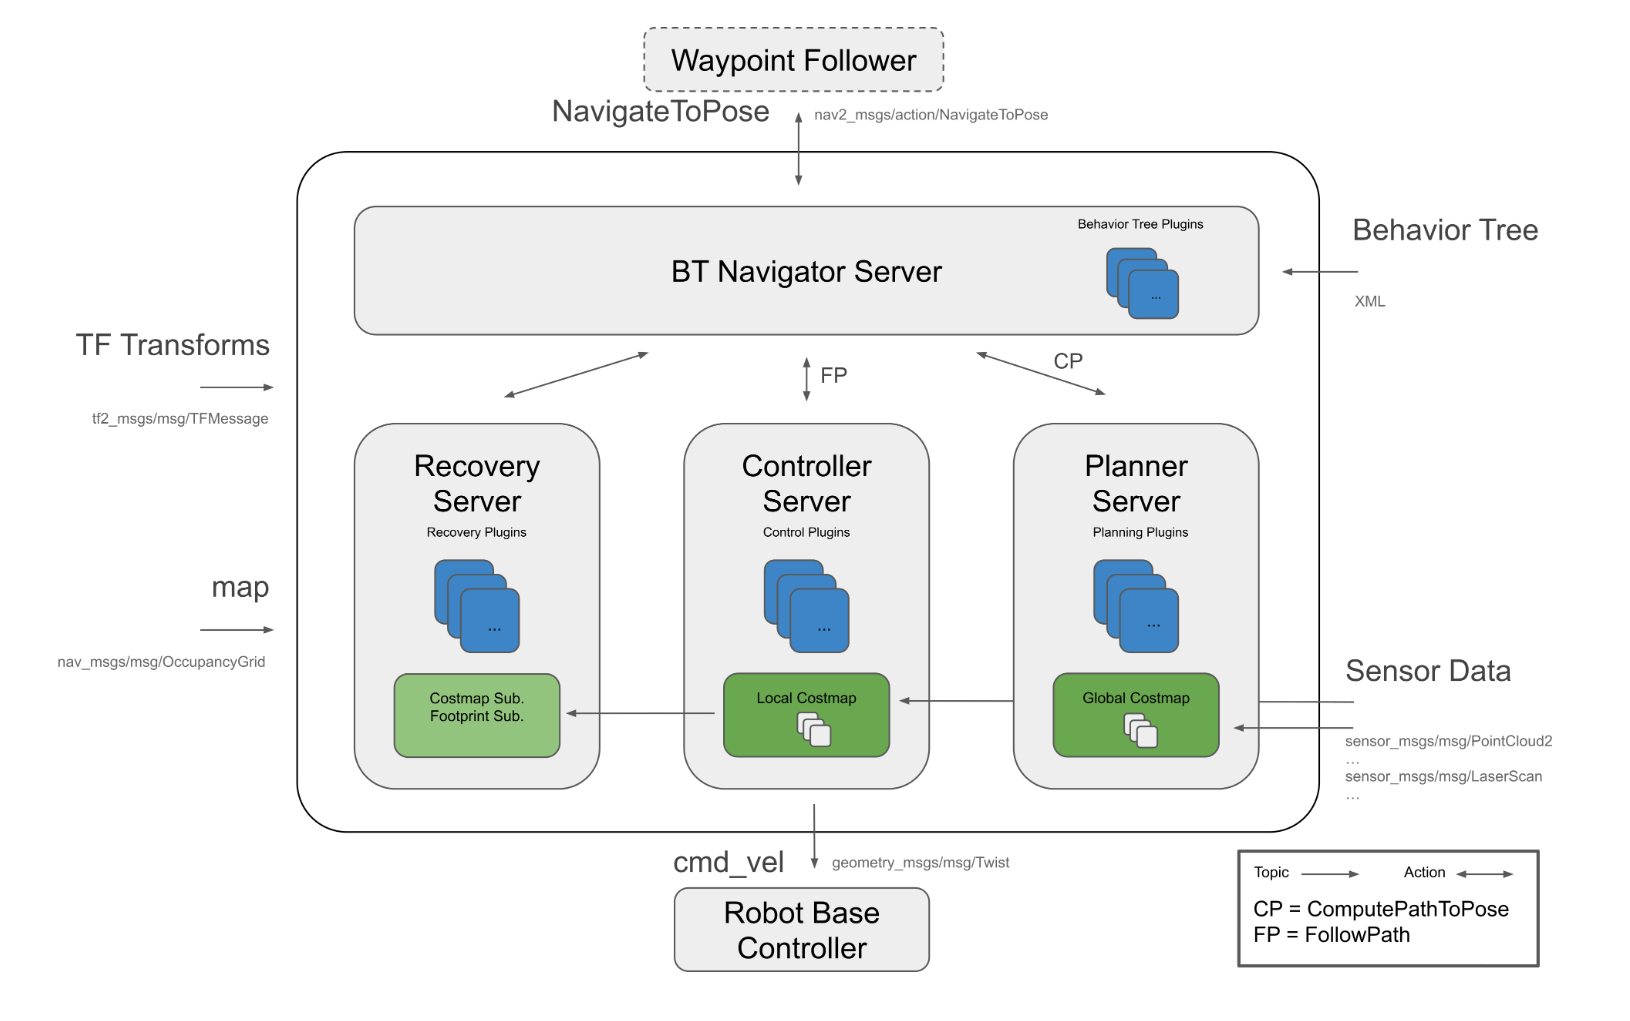
\includegraphics[width=0.8\textwidth]{./images/Nav2导航框架.png}
    \caption{Nav2导航框架}
    \end{figure}
从上面可以看出,导航需要:

\textbf{[1]地图(全局代价地图Global Costmap)}

\textbf{[2]导航系统(全局规划器Global Planner)}

\textbf{[3]定位系统(多传感器融合定位)Sensor Transform}

\textbf{[4]附近的视野(局部代价地图Local Costmap)}

\textbf{[5]车手(局部规划器Local Planner)}

\textbf{[6]应急方案(恢复行为树Recovery Behavior Tree)}

因此,导航的工作流程就是:

通过传感器数据与全局地图匹配,获得自身在地图的坐标;
根据目标坐标,利用全局规划器算出路径;
实时更新自身定位,并将扫描到的障碍物信息融合到局部代价地图中;
根据局部代价地图,利用局部规划器算出车各个方向的速度应该是多少,发给下位机;
如果遇到特殊情况则进入恢复行为树,暂停部分服务,直到脱离特殊情况;
根据规定的时间间隔(或情况),重新获取定位和目标,规划全局路径,并一直循环。